\chapter{Рудная Радунка}

А 13 марта 2016 года мы отправились в краеведческую вылазку, дабы изучить Рыжую речку под Выгуровщиной. Как выяснилось позже, все фотографии, сделанные мною в тот день в промежуток времени вылазки (однако не после) странным образом не сохранились на карте памяти мобильного телефона, хотя за день до этого всё снималось, и по возвращении домой тоже. Отмечу также, что фотографировать 13 марта я начал не прямо под Выгуровщиной, но раньше, еще в кварталах около бульвара Перова. Эти снимки тоже не сохранились.

Что же, громко разговаривая при сильном ветре и шумной трассе, мы пересекли огороженную линию скоростного трамвая и приступили к изучению местности. Прошли через поле к линии тополей, растущих вдоль русла Рыжей речки. Стану тут величать ее Рыжая с большой буквы, раз уж в истории имя ее потерялось, хотя быть может оно и упомянуто в земельных документах, которые я приводил в прошлой главе.

Впадает речка в Черторыю, точнее, вытекает из нее\footnote{Место впадения: 50°30'2"N  30°34'8"E, канал оттуда прослеживается примерно до 50°30'14"N 30°34'37"E.}. Сейчас Рыжая наполовину запитана водой из Черторыи и посему может считаться заливом. Половина же ее русла – пересохшая. 

Мы двигались по течению, стало быть от Черторыи прочь. Берега вначале были низкие, потом выросли чуть ли не до трех метров, и Рыжая протекала там будто по рву между высокими валами. Изгибы русла кое-где под прямым углом. Всё это свидетельствует о рукотворности если не самого русла, то его очертаний.

Вода несет рыжие частицы, они заилили собой всё дно и берега, так что на вид речка на большей части своей протяженности – рыжая. К руслу примерно с севера подходит пустой ров, и около речки образуется эдакий сухопутный прямоугольный (при виде сверху) островок, одной стороной примыкающий к Рыжей, а четырьмя глядящий в поле.

\begin{center}
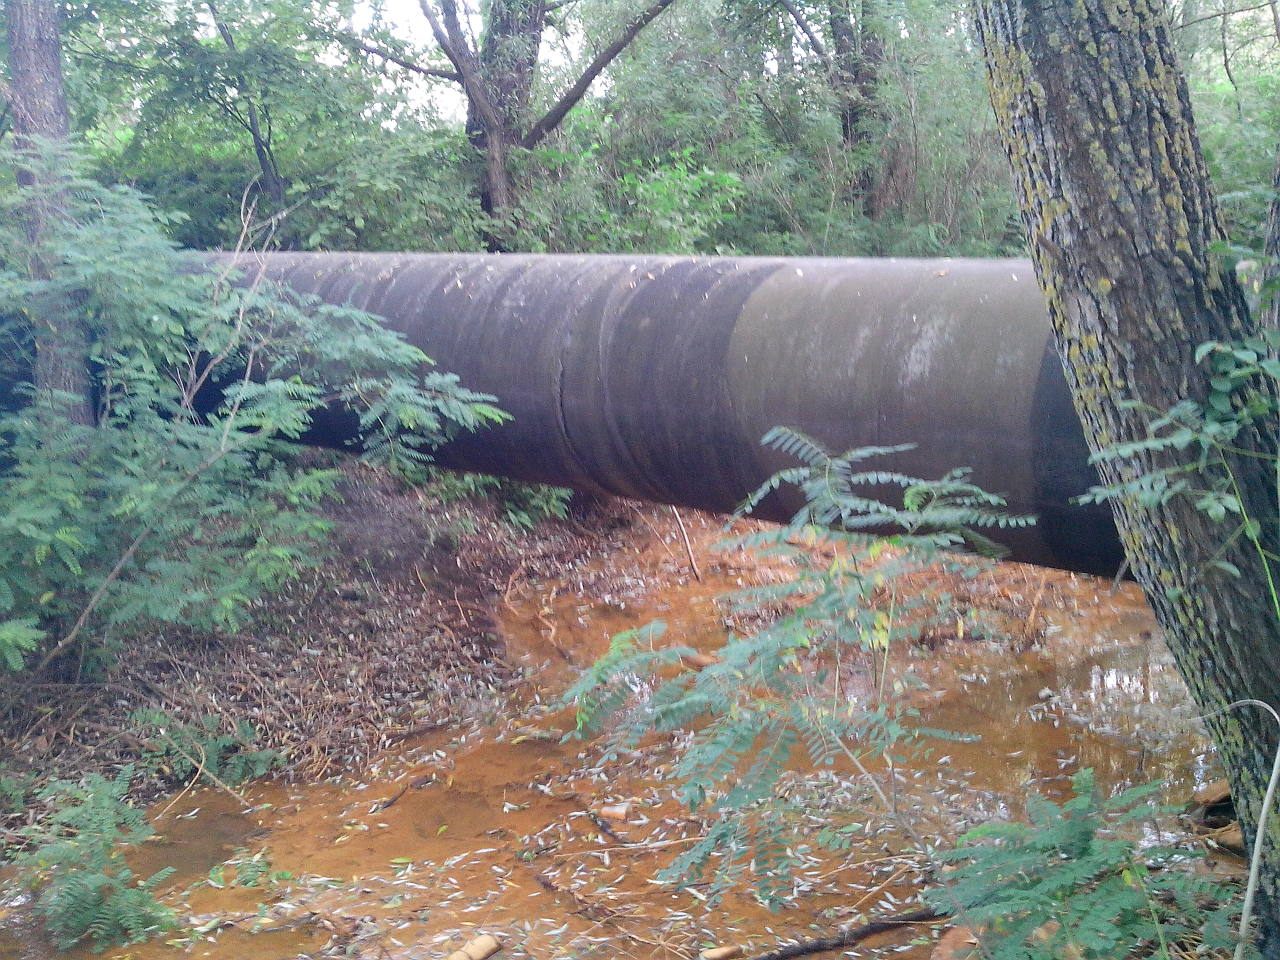
\includegraphics[width=\linewidth]{chast-gorodki/rud/s_IMG_20140806_140003.jpg}

\textit{Для переправы служит труба. 2014 год.}
\end{center}

По полю – а это поле к западу и южнее озера Гнилуши – всюду виднеются то остатки невысоких теперь валов, то довольно глубокие сухие каналы неизвестного происхождения.

Метрах в трехста южнее озера Гнилуши, Рыжая уже представляет собой пересохшее русло. С востока к нему присоединяется еще какой-то плохо обозначенный, однако с бетонным желобком канал.

Чуть севернее, овраг русла Рыжей примыкает к круглому входу в бетонный коллектор, в котором журчит и падает с высоты вода, однако наружу в поверхностное русло она не поступает и вероятно течет каким-то подземным путем. Это, если не ошибаюсь, к юго-западу от девятых домов по улице Димитрова.

На векторной карте Визикома 2006 года вся речка обозначена синим, и от существующего в 2016 году портала коллектора у Выгуровщины продолжается к северо-западу, вдоль улицы Бальзака, почти до собора святой Троицы на перекрестке улиц Рыбака, Полевой и Бальзака.

Однако на спутниковой карте того же 2006 года русла там не заметно, равно как на аэрофотоснимках 1943 года (когда рельеф был совсем уж другим) – следовательно, карта Визикома 2006 года отражает некий канал, существовавший после 1943 года и опущенный под землю до 2016-го.

Прежде чем рассказывать дальше, необходимо коснуться вопроса взаимного расположения речки Радунки, русла Рыжей речки и Прудка. 

Радунка, если озеро Гнилуша – ее часть, по сопоставлению с местностью, должна была бы пересекать Рыжую, поскольку южная оконечность озера Гнилуши примерно подходит к месту, где начинается русло Рыжей около входа в коллектор.

Реки друг друга не пересекают, значит русло (либо части) Рыжей возникло позже времени существования Радунки как цельной реки, или же в ее время, но в качестве канала.

На карте лоций 1914-го, примерно по руслу западной половины Рыжей речки, от Прудка в Выгуровщине, с востока на запад идет прямой канал до устья современной Рыжей речки. 

Возможно, этот канал существовал издавна и показан на карте 1719. Отличие его от русла Рыжей речки – Рыжая заворачивает на север к Гнилуше, а канал следовал к Прудцу.  

Рассмотрим фрагмент этой карты.

\begin{center}
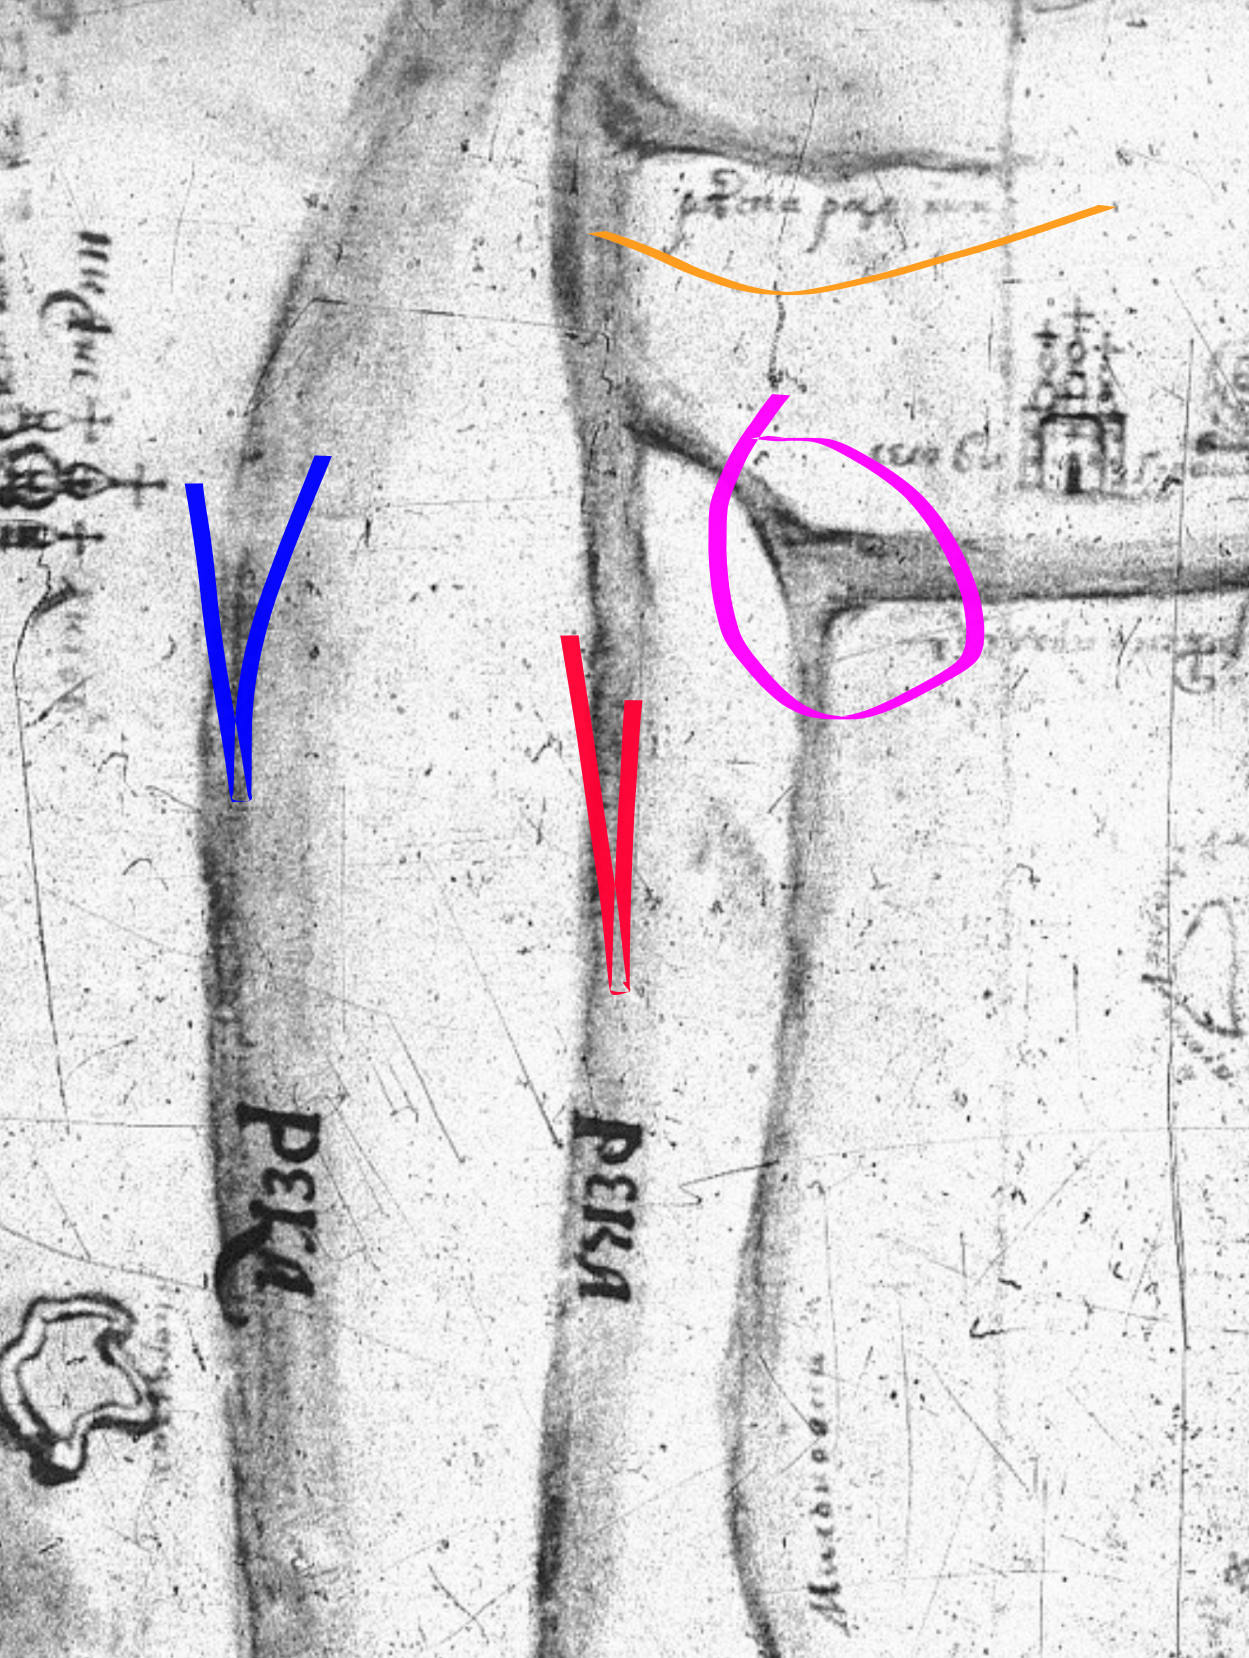
\includegraphics[width=\linewidth]{chast-gorodki/rud/1719-cross.jpg}
\end{center}

Синим я пометил Днепр, красным – Черторыю, оранжевым – некий приток, подписанный возможно как «речка радунка», наконец малиновым – развилку «реки Пруд» (река подходит справа) около села Выгуровщины, там изображена церковь. Одно русло оттуда идет в Черторыю, другое на юг, обозначено как «речка М....» и дальше этого «м» я не могу разобрать. Русло от «реки Пруда» к Черторые просится на роль канала с карты 1914 года, а заодно и южной части Рыжей речки.

На карте РККА 1930-х и немецких аэрофотоснимках 1943 года тоже прослеживается южная часть русла Рыжей речки (сдвинутая чуть южнее современной при наложении изображений), вероятно соответствующая каналу из Прудца в Черторыю на карте 1914 года, вплоть до устья, которое было выдвинуто более на запад относительно 2016 года.
%(довольно глубокие, с берегами высотой около 3,5 метров).  

%В 1943 году русло около устья в Черторыю расположено несколько южнее, и нынешнее повторяет его очертания до половины Рыжей, однако смещено севернее. Само устье «старого» русла выдвинуто на запад, вместе с сушей, которая затем исчезла. 

Считаю, что русло Рыжей речки частично прорыто после 1943 года, однако по различным старым руслам на местности – по крайней мере по каналу от Прудка к Черторые, да поперек Гнилуши, и возможно по давним глубоким рвам.

В современном русле Рыжей речки происходит образование болотной руды. Ее следы находим в окрестностях повсюду в виде россыпей, вероятно раздробленных человеком в подготовке к выплавке в печи. О главной нашей находке я поведаю чуть позже. 
\vspace*{\fill}
\begin{center}
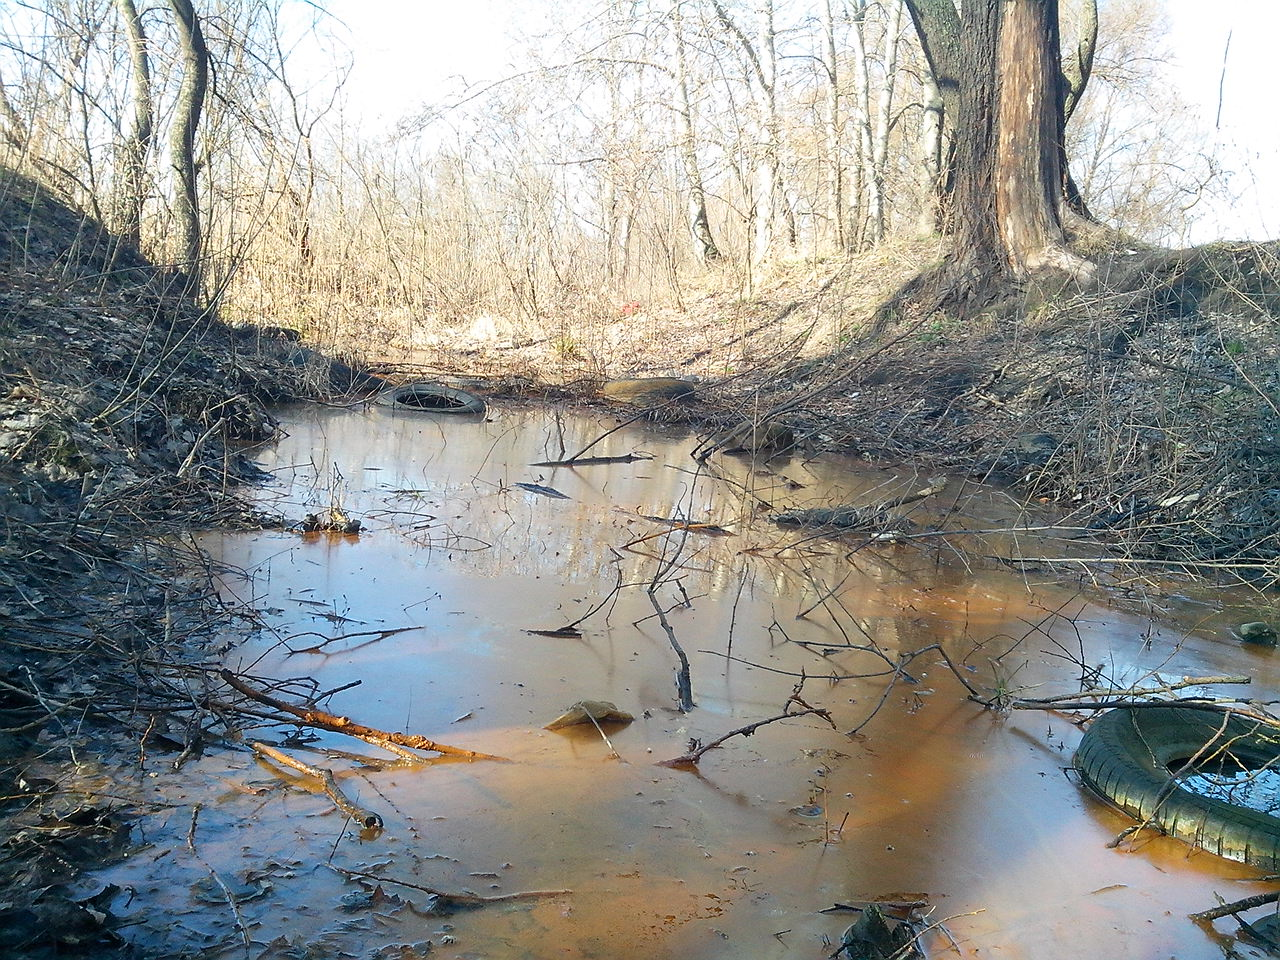
\includegraphics[width=\linewidth]{chast-gorodki/rud/IMG_20160316_145507.jpg}
\end{center}
\vspace*{\fill}

\newpage
\vspace*{\fill}
\begin{center}
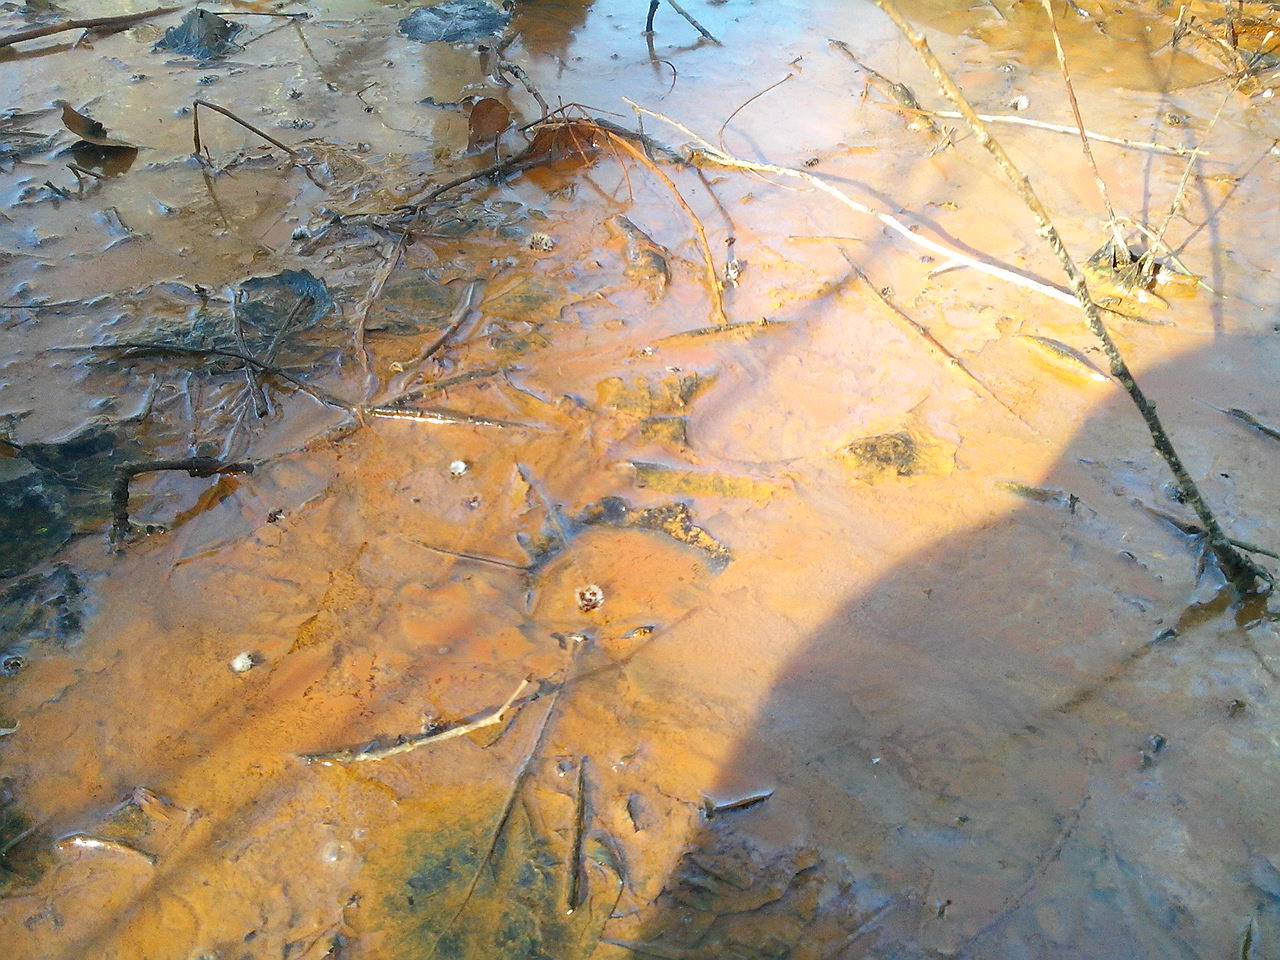
\includegraphics[width=\linewidth]{chast-gorodki/rud/IMG_20160316_145454.jpg}
\end{center}

\begin{center}
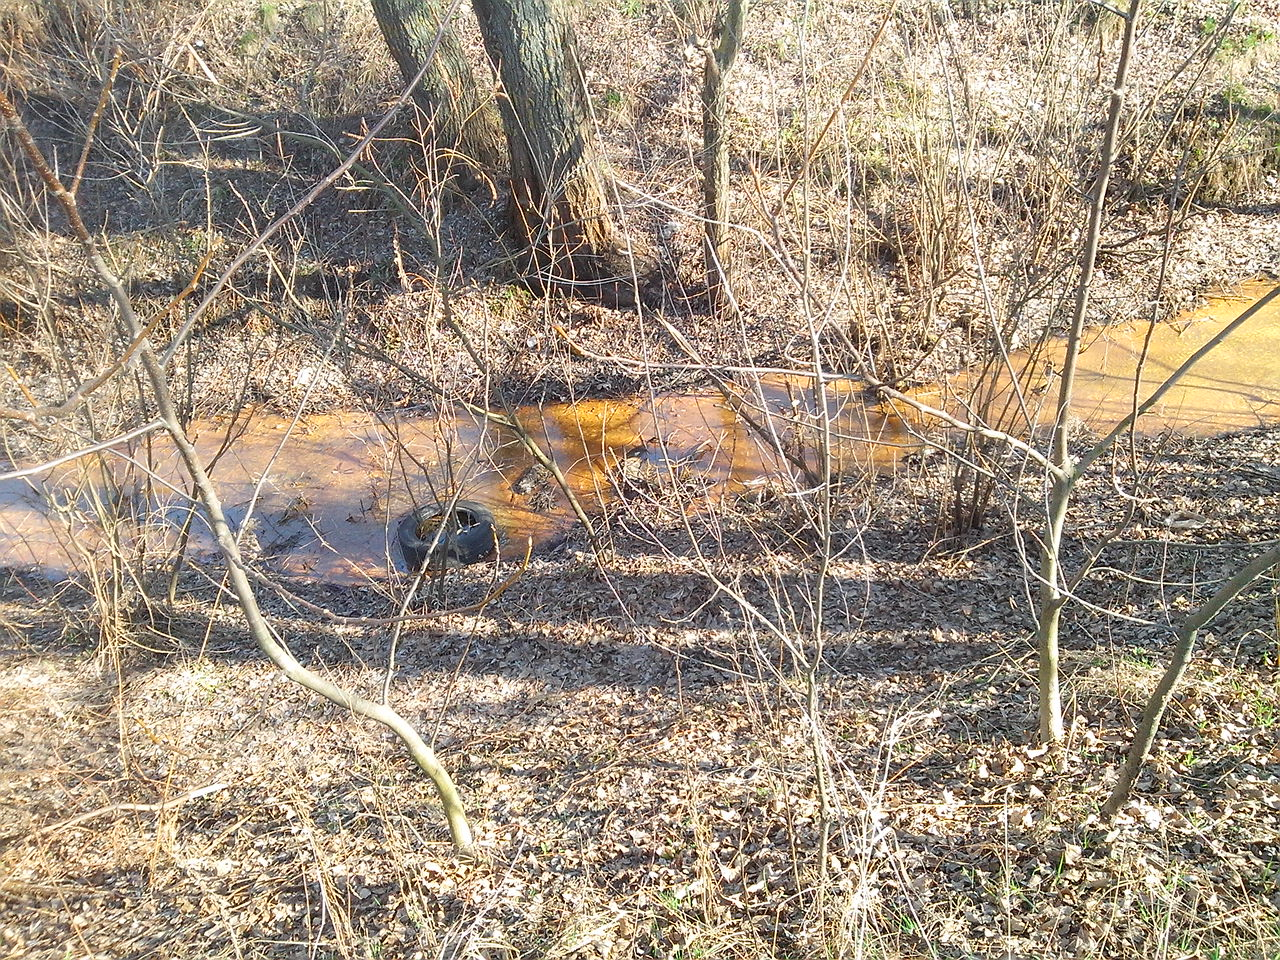
\includegraphics[width=\linewidth]{chast-gorodki/rud/IMG_20160316_145834.jpg}
\end{center}
\vspace*{\fill}
\newpage

Рыжий цвет присущ окисленным частицам железа. Они могут окисляться водой либо бактериями. Атомы окисляющегося вещества теряют электроны. Обратное действие называется восстановлением, когда электроны присоединяются от другого вещества (оно в свою очередь окисляется, теряя электроны). Знаменитая ржавчина – тоже окись железа.

Вода рыжей речки насыщена рыжими частицами. Ими же покрыто всё дно, попавшие в воду ветки, даже листья вербы. Эти окисленные частицы – продукт жизнедеятельности железобактерий, живущих в воде. Чем именно они питаются – бог весть, я не знаю, колония каких именно бактерий поселилась у околиц Выгуровщины. Но именно эти микроскопические ребята выдают окисленные частицы железа, которые оседают на дне. Так рождается болотная руда – бурый железняк, он же лимонит. Вплоть до 18 века это сырье использовалось в металлургическом производстве.
\vspace*{\fill}
\begin{center}
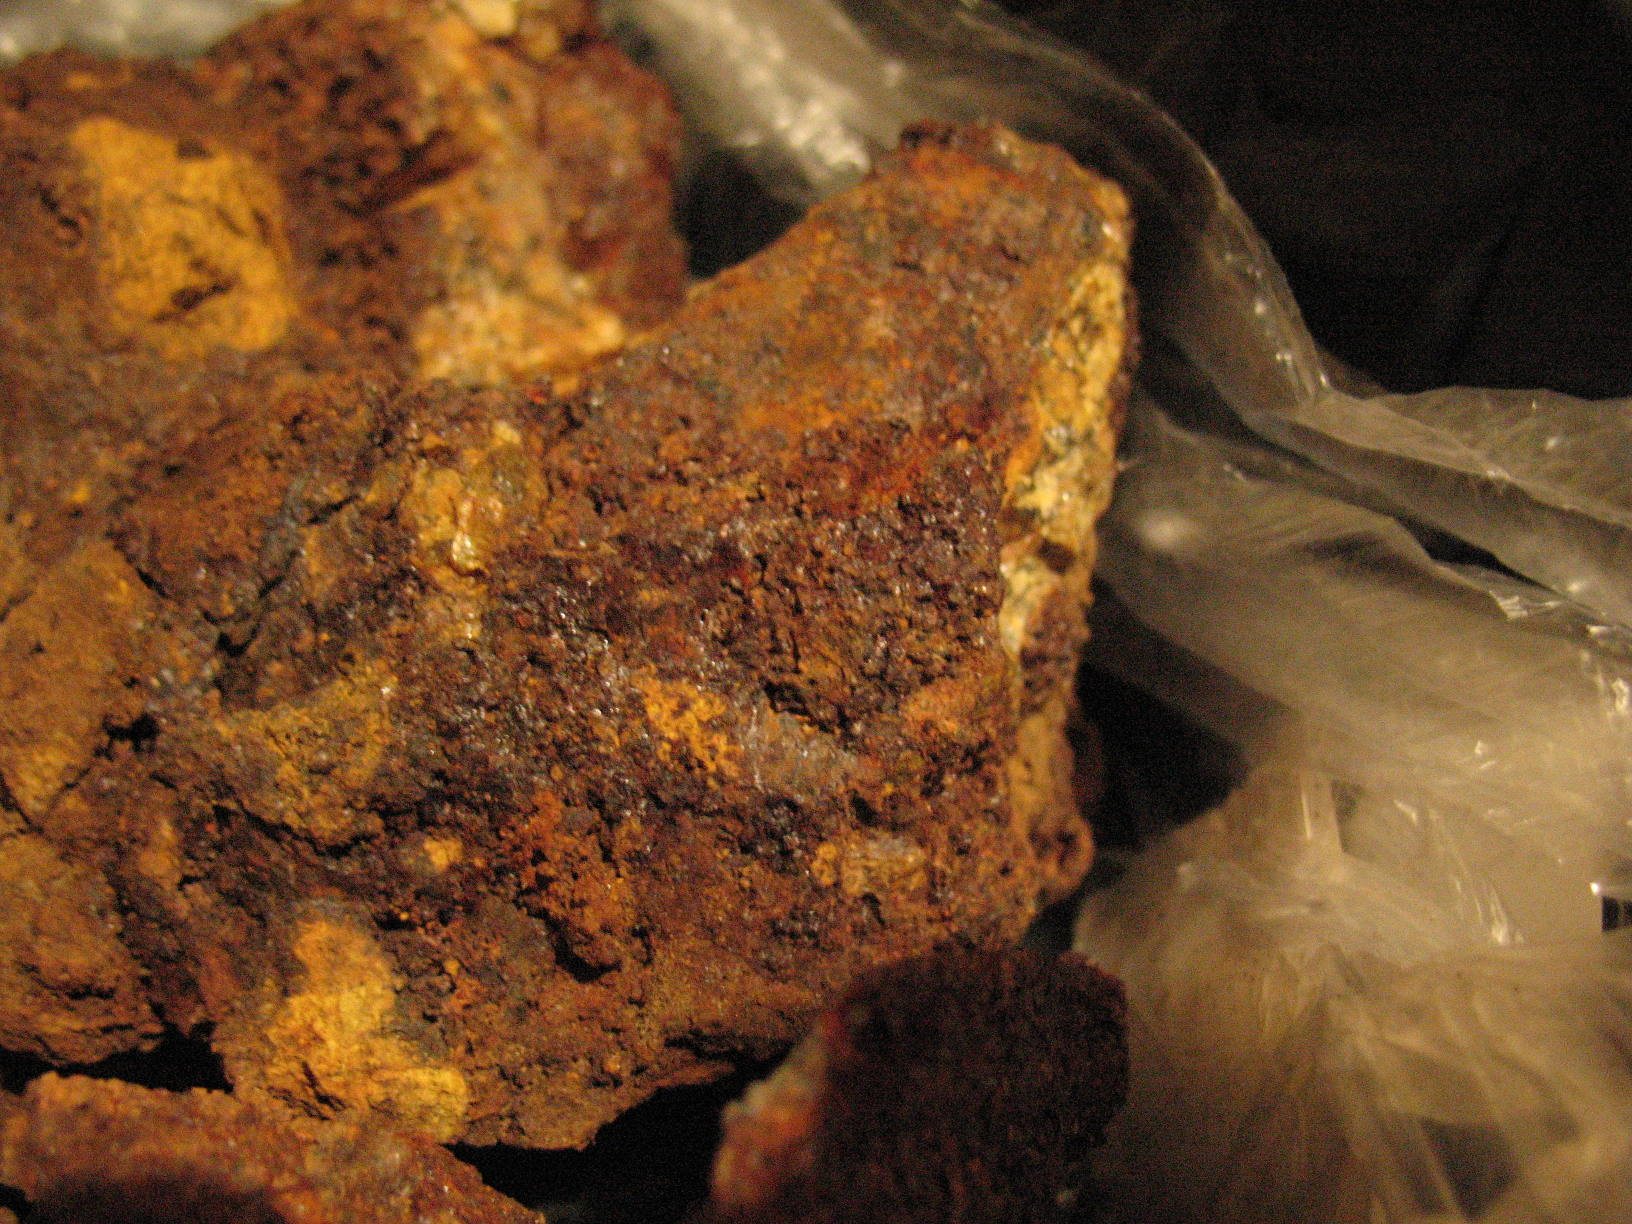
\includegraphics[width=\linewidth]{chast-gorodki/rud/s_IMG_4468.JPG}

\textit{2016. Найденный у Выгуровщины кусок болотной руды.}
\end{center}
\vspace*{\fill}
\newpage

Железная руда – собирательное название пород, содержащих железо. Лимонит, железистый песчаник – лишь одни из них, однако наиболее доступные для добычи в давнее время, и наиболее простые в выплавке. Сейчас в качестве руды используют другие породы.

Неподалеку от современного начала русла Рыжей речки, у рощицы близ прерывающегося невысокого валка, мы нашли место древней переработки руды.

\begin{center}
\includegraphics[width=0.93\linewidth]{chast-gorodki/rud/\myimgprefix IMG_20160405_135659.jpg}

\textit{2016. Вот прямо здесь.}
\end{center}

\newpage

Большие осколки гранита, которым было выложено дно плавильной печи – горна, остатки шлака, куски самой руды и крицы. К собранным образцам «липнет» магнит, с разной силой в зависимости от степени содержания частиц железа в образце.

Также мы провели замеры магнитометром, встроенным в смартфон. Уровень магнитного поля окружения показывал 49-51 нанотесла. При поднесении смартфона к месту переработки металла уровень поднимался до 69. Это мы замеряли, посетив  околицы Выгуровщины повторно, через несколько дней. Тогда же сняли нашу вылазку для очередной серии «Киевской амплитуда», с заголовком «Под Троещину за рудой».

\begin{center}
\includegraphics[width=\linewidth]{chast-gorodki/rud/\myimgprefix IMG_20160405_140344.jpg}

\textit{2016. Вал, за которым перерабатывали руду.}
\end{center}

Поскольку в Рыжей речке поныне действует колония железобактерий, а обнаруженным нами следам переплавки руды – сотни лет, предположу, что в давнее время эта местность являлась рудником – источником болотной руды – и здесь же перерабатывалась. 

Не относится ли к этому уже известные нам строки из статьи Завитневича? Напомню. Около погребального вала было вот что:

\begin{quotation}
Под насыпью, на почвенном слое, оказалось огнище. Начинаясь в центре, оно наполняло собою весь юго-восточный угол отведенной для изследования площади и находилось, кажется, на самом возвышенном пункте озернаго берега. Огнище это, мало походило на те кострища, с которыми археологам приходится встречаться в курганах с трупо-сожжением: оно было следствием действия сильнаго и продолжительнаго огня. О силе огня можно заключать из того, что многие предметы не только медные, но и железные, совершенно разложились и, смешавшись с песком, образовали целыя труды безформеннаго сплава. 
\end{quotation}

То, что мы – выходит, неподалеку от «городища» Завитневича – нашли не части этого «бесформенного сплава», но именно место выплавки, доказывается кусками гранита, коим выкладывалось дно печи. Однако закономерен вопрос – не является ли «огнище» Завитневича тоже местом металлургического производства? Он упоминает также некие расплавившиеся готовые уже предметы, как их трактовать, я не знаю.

Но теперь и названия Радосынь, Родунь, Радунка получают некоторую привязку к словам «рудой», «руда». Однако и «погребальное» толкование весьма сильно.

5 апреля 2016 года я открыл для себя начало велосезона очередным посещением окрестностей рыжей речки. Теплынь под двадцать градусов, на голубом небе ни облачка. На Радужном массиве вознамерились расцветать марельки.

Сначала я поехал к известному месту обнаружения переработки руды, чтобы набрать еще образцов. Неподалеку в траве сидели пожилые да пьяные, хором нескладно пели. Рядом грунтовкой шел молодой пьяный и говорил по мобилке. Немного дальше на дороге шатались две тетки, тоже пьяные. Они упали, лежали на спине и громко смеялись.

Я принялся ковыряться в железном шлаке, шарить по траве – оказалось, что столь явно выраженный прямоугольник руды и шлака продолжается, он расползся за видимые границы, скрытый листьями и травой. Сфотографировав всё внизу и вокруг в разных ракурсах, я сел на велик и принялся колесить по тропам и грунтовкам в поле, сплошь утыканном буграми, валами, следами старых русел.

Метрах в трехста от найденной в прошлую вылазку руды я приметил бугор, поврежденный грунтовкой. Рыжее! Направился туда, положил велик у обочины, вытащил магнит для проверки.

Снова – следы обработки железа! Куски руды, шлака, пачкающие руки желтым разбитые стенки глиняного горна с прилипшим к ним опять же шлаком. Произведенный здесь предмет – некая ржавая штучка, похожая на гирьку.
\vspace*{\fill}
\begin{center}
\includegraphics[width=\linewidth]{chast-gorodki/rud/\myimgprefix IMG_20160405_141355.jpg}

\textit{2016. Руда.}
\end{center}
\vspace*{\fill}
\newpage

\begin{center}
\includegraphics[width=0.98\linewidth]{chast-gorodki/rud/\myimgprefix IMG_20160405_141828.jpg}

\textit{2016. Обломки горна.}
\end{center}


\begin{center}
\includegraphics[width=0.98\linewidth]{chast-gorodki/rud/\myimgprefix IMG_20160405_141648.jpg}

\textit{2016. Крошки от руды притягиваются обычным магнитом с холодильника.}
\end{center}

\begin{center}
\includegraphics[width=\linewidth]{chast-gorodki/rud/\myimgprefix IMG_20160405_142303.jpg}

\textit{2016. Вид с места находки примерно на юго-запад.}
\end{center}

И через день получаю сообщение от Константина Чимбая, которому месяц назад, на собрании краеведческого клуба «Кияне», передал кусочек руды (с малым содержанием железистых частиц, ибо лучший из имеющихся с собой кусков я оставил при себе) для анализа в фи\-зи\-ко-химической лаборатории:

\begin{quotation}
Найденный образец породы притягивался к магниту, имел характерный ржавый цвет и пористую структуру. Анализ, проведенный физи\-ко-химической лабораторией, показал, что образец содержит 18\% окиси железа, примеси закиси железа, окись марганца и фосфаты. Данный анализ свидетельствует о том, что найденный образец является бурым железняком органического происхождения, или другими словами, болотной (луговой) рудой.
\end{quotation}

Это подтвердило мое мнение, что мы нашли болотную руду. В чем я впрочем не сомневался.

Что же?

Погребальный вал и следы металлургии у него. Описанные мною в этой главе следы металлургии в двухста метрах на юг от современного южного конца Гнилуши, а значит и от погребального вала. Еще несколько «городищ», вычисляемых по разным источникам и очевидных на местности, как например на западном берегу Гнилуши.

Не слишком ли много всего древнего для одного места? Это место надо сделать заповедником и осторожно изучать. Однако его перекроили каналом, застраивают, а ученые повторяют уже несколько веков кряду – летописный Городец и замок Олельковича! 

Кстати, по берегам Рыжей речки и в поле мне попадались, по одной и рядами, прямоугольные ямы разной глубины, эдакие могилки, размером годные для захоронения с скорченном положении. Судя по всему, этим раскопам 10-15 лет.

Местные жители утверждают, будто ямы вырыты школьниками. Но школьников часто привлекают к раскопкам археологи.

По одним сведениям, школьники занимались рытьем «могилок» на занятиях по допризывной подготовке, по другим сведениям, школьники рыли там не «могилки», но некие рвы – я не могу проверить это и посему не доверяю таким сообщениям, однако привожу их здесь.

К югу от русла Рыжей речки на спутниковых снимках поныне просматриваются части огромного сердца. Это, судя по газетной публикации в «Сегодня», в 2009 году там высадили в определенном порядке деревца, чтобы попасть в Книгу рекордов Гиннесса.
 
Однако прямоугольные ямы попадались нам к северу от русла, причем глубиной зачастую более, чем у лежачего окопа, если б это были окопы.

Что до высаженных в форме сердца сотен деревьев, я их не видел, да и ямы под саженцы рыли бы круглые и не такие глубокие.

Но металлургия. Может быть здесь под Выгуровщиной была древняя промзона – добывалась и обрабатывалась руда. Объем производства? А кто скажет? Никому дела нет, удивительно что в 2016 году еще не застроили поле на запад от Гнилуши. Тут металл, там – на Кирилловских высотах и Оболони – тоже металл – вот и славился давний Киев производством мечей, известных даже Арабам.

Производственное, металлургическое значение окрес\-тностей Выгуровщины может дополнять вероятное значение обрядовое, священное.

Мы знаем из летописи, что был «скотий бог» Волос, с Перуном связываем гром и молнию, но если металлургия была таким важным делом в Киеве, то должны были почитать некоего бога-кузнеца, и возможно существовал его храм или святилище. Таковой поганский бог в летописях не упомянут, либо если упомянут, то не указана его профессия.

Кто такие были Сварог, Семаргл или Мокошь? Ничего, кроме имен, о них не сохранилось. Разве что в Ипатьевской летописи Саварог или Сварог было другое имя египетского правителя Феоста, в третьем поколении после Великого Потопа и разделения языков. Летопись пересказывает «Фронограф» – Хронограф Георгия Амартола, а возможно еще какие-то источники:

\begin{quotation}
поча царствовати первое Местром от рода Хамова, по нем Еремия, по нем Феоста, иже и Саварога нарекоша Егуптяне
\end{quotation}

При этом Свароге, 

\begin{quotation}
в время царства его, спадоша клеще с небесе, нача ковати оружье, преже бо того палицами и камениями бьяхуся
\end{quotation}

Во время царствования Сварога в Египте, с неба упали клещи, и люди начали ковать оружие, а прежде того бились палицами и камнями.

Феост-Сварог установил закон – на одного мужа по одной жене, одной жене по одному мужу,

\begin{quotation}
аще ли кто переступить, да ввергнуть и в пещь огнену. Сего ради и прозваша и Сварогом и блажиша и Егуптяне.

И по сем царствова сын его, именем Солнце, егоже наричуть Дажьбог [...]
\end{quotation} 

Я опускаю обширный летописный рассказ о египетских правителям Свароге и Дажьбоге, возможно известных нам под именами каких-то фараонов. Был же во Франции Людовик, «король-солнце», только его не обожествляли.

Летопись толкует прозвище Феоста – Сварог – как произошедшее от ввержения преступников в печь, где они вероятно варились, сваривались, потому Сварог.

Краткая заметка про упавшие с неба клещи позволяет сделать вывод о том, что при Свароге «с неба» людям была дана технология по крайней мере ковки металла, если не весь металлургический процесс (добыча руды и ее выплавка).

Кузнецов более близкого к нам времени, допустим 19 века, связывали с нечистой силой, с чертом – стало быть с теми же поганскими богами.

%Конечно, проще рисовать местных жителей-полян полудикими дурнями, приносящими дань стопками шкур или какими-нибудь лаптями. 
